%\hypertarget{actividades}{} 

%\section*{\centering \textbf{Actividades}}
%\addcontentsline{toc}{section}
%{\protect \numberline{I. }Actividades} 
% \rule{\textwidth}{0.4pt} % Línea horizontal 
%\label{intro}
%\input{Components/Activities}


\textbf{\textit{Abstract}} - Este artículo presenta el desarrollo y la evaluación de un entorno educativo gamificado en Roblox, diseñado específicamente para la enseñanza práctica de metodologías de aseguramiento de calidad de software (QA). El sistema, denominado "Shop \& Jump Simulator (Bug Edition)", implementa una arquitectura modular con errores lógicos intencionales en sus subsistemas de economía, progresión y sincronización multijugador. El objetivo principal es proporcionar a los estudiantes un escenario controlado donde puedan aplicar niveles de prueba manual, unitaria, de integración y automatizada mediante el uso de TestService. Los resultados demuestran que la exposición a fallos distribuidos y flujos de integración rotos fortalece la capacidad diagnóstica del alumno, permitiendo identificar vulnerabilidades críticas como saldos negativos, inconsistencias en multiplicadores de recompensa y falta de validación en la comunicación cliente-servidor.

Todos los códigos fuente, se encuentran dentro del repositorio del proyecto, el cual se encuentra disponible en GitHub: \url{https://github.com/ArelyX1/TestingUCSM/tree/master/F1/Teo1}.  
\vspace{0.5em}

\textbf{\textit{Index Terms}} - Software Testing, Unit Testing, Integration Testing, Test Automation, Gamification, VS Code

\section{Introducción}
\label{intro}
La creciente complejidad de los sistemas de software modernos exige que los estudiantes de ingeniería no solo comprendan la teoría del testing, sino que también desarrollen habilidades prácticas para identificar fallos en entornos dinámicos y distribuidos. En este contexto, el uso de plataformas de desarrollo de juegos como Roblox Studio ofrece una oportunidad única para simular arquitecturas cliente-servidor reales donde los errores de lógica y sincronización son comunes. El presente informe detalla la implementación de un mini-juego educativo, denominado \"Shop \& Jump Simulator (Bug Edition)\", que integra módulos de estadísticas de jugador, sistemas de tiendas y mecánicas de salto, todos ellos vinculados a un motor de economía que presenta comportamientos erráticos diseñados para el aprendizaje \cite{ucsm}.

Para elevar este ejercicio a un estándar profesional de ingeniería, el flujo de trabajo se integró con Visual Studio Code utilizando Dev Containers, lo que permitió un entorno de desarrollo estandarizado y aislado para la ejecución de pruebas. El núcleo de la validación técnica se apoyó en el plugin Busted Test Explorer, facilitando la gestión y visualización de los tests unitarios y de integración de manera eficiente. Este enfoque permitió explorar cómo pequeñas fallas en el código de un módulo, como la falta de validación de fondos en el ShopSystem, pueden escalar hasta corromper el flujo completo de la aplicación, obligando al evaluador a transitar desde la observación empírica del testing manual hasta la rigurosidad técnica de la automatización.

Finalmente, el proyecto busca cerrar la brecha entre el aula y la industria mediante la simulación de un ciclo de vida de desarrollo de software colaborativo. Al dividir a los participantes en roles de testing manual, automatización y desarrollo de backend, se fomenta un entorno donde la resolución de conflictos de integración y la gestión de regresiones son elementos centrales del aprendizaje. La introducción de bugs distribuidos asegura que los estudiantes comprendan que el cliente no es una fuente confiable y que la validación en el servidor es indispensable para garantizar la integridad de cualquier sistema multiusuario.


\section{Módulos iniciales del proyecto}
\label{workflow}
Ahora se presenta el desarrollo de los módulos iniciales del proyecto, que incluyen la implementación de un sistema de estadísticas de jugador, un sistema de tienda y un sistema de salto, todos ellos integrados en un motor de economía diseñado para presentar comportamientos erráticos. Estos módulos fueron desarrollados utilizando Roblox Studio, con el objetivo de simular un entorno cliente-servidor realista donde los errores comunes pueden ser identificados y corregidos a través de pruebas manuales y automatizadas.

Para los testeos se utilizó Visual Studio Code con Dev Containers, lo que permitió un entorno de desarrollo estandarizado y aislado. El plugin Busted Test Explorer facilitó la gestión y visualización de los tests unitarios y de integración, permitiendo a los evaluadores identificar rápidamente las fallas en el código y comprender cómo estas afectan el flujo general de la aplicación.


\newpage
\begin{strip}
    \centering
    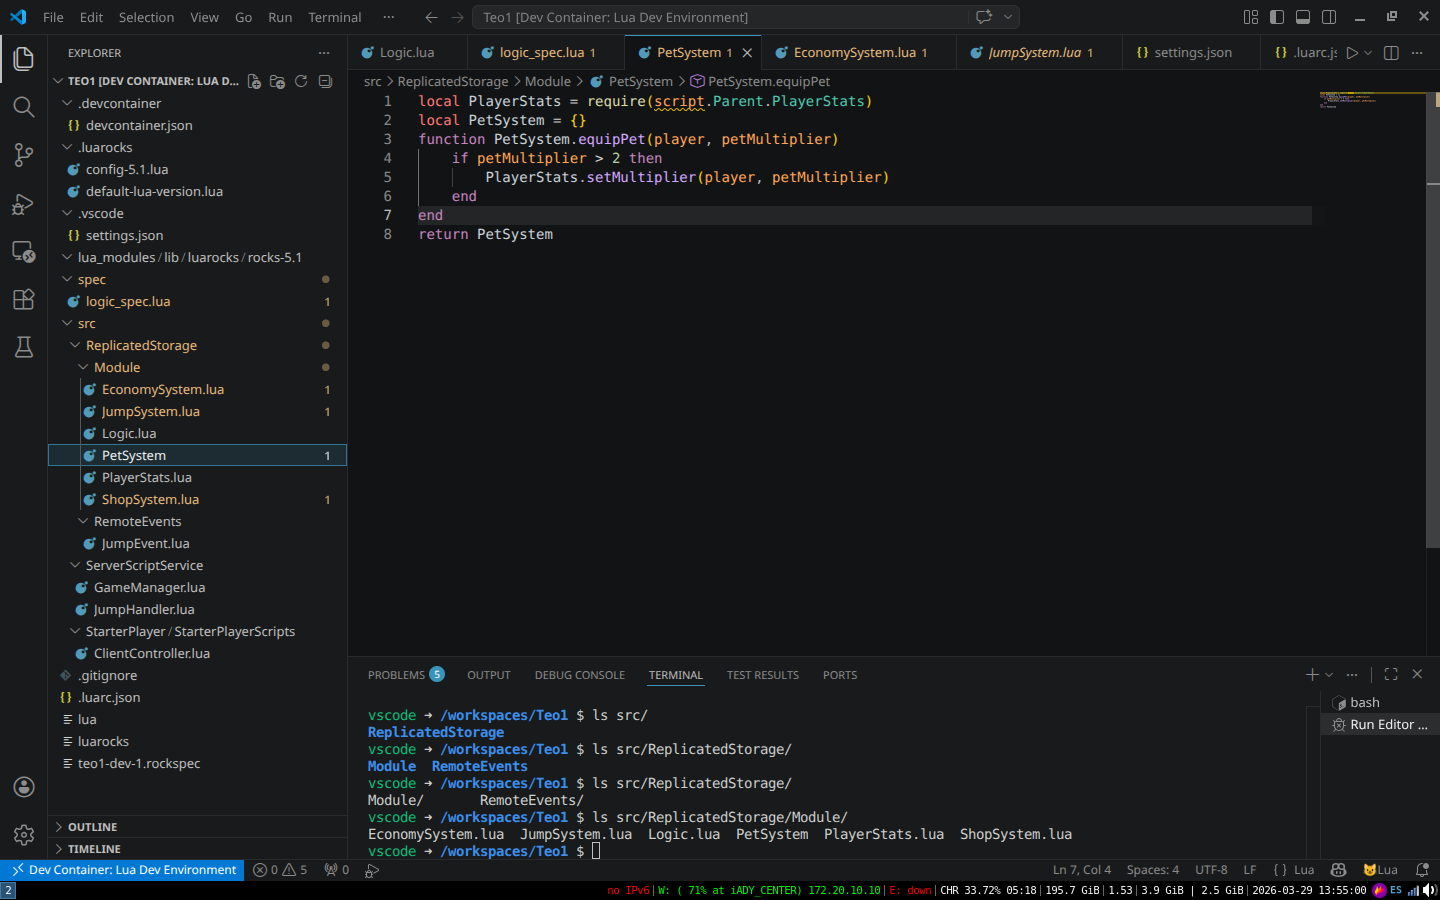
\includegraphics[width=1\textwidth]{media/FigGeneral/1.png}
    \captionof{figure}{Workspace de Visual Studio Code con Dev Containers}
    \label{fig:workflow_isometrico}
\end{strip}

Como se visualiza en la \cref{fig:workflow_isometrico}, el entorno de desarrollo se configuró para permitir la ejecución de pruebas unitarias y de integración de manera eficiente. Esto facilitó la identificación de errores en los módulos desarrollados, como se muestra en los siguientes apartados donde se detallan los bugs encontrados y las soluciones implementadas para cada módulo. Se muestra la estructura del proyecto, con los módulos principales y los archivos de prueba correspondientes, lo que permitió un flujo de trabajo organizado y efectivo para el desarrollo y la validación del sistema.
La extención de Dev Containers permitió crear un entorno de desarrollo aislado, lo que garantizó que las pruebas se ejecutaran en un entorno controlado, evitando conflictos con otras configuraciones del sistema. Esto fue crucial para asegurar la reproducibilidad de los tests y la confiabilidad de los resultados obtenidos durante el proceso de desarrollo.
Se instalo Lua y el plugin Busted Test Explorer, lo que permitió ejecutar los tests unitarios y de integración directamente desde Visual Studio Code, facilitando la identificación de errores y la validación de las correcciones implementadas en los módulos del proyecto. Esta integración mejoró significativamente la eficiencia del proceso de desarrollo y testing, permitiendo iterar rápidamente sobre el código y asegurar su calidad antes de la implementación final en Roblox Studio.
Además, se configuró el entorno para permitir la ejecución de pruebas automatizadas, lo que permitió validar la funcionalidad de los módulos de manera sistemática y consistente, asegurando que cualquier cambio en el código no introdujera nuevos errores o regresiones en el sistema. Esta configuración fue esencial para mantener la calidad del código a lo largo del desarrollo y garantizar que los módulos funcionaran correctamente en conjunto dentro del entorno de Roblox Studio.

El primer módulo desarrollado fue el sistema de estadísticas de jugador (PlayerStats), que se encargaba de gestionar la experiencia y el nivel del jugador. Se implementó un test unitario para validar la funcionalidad del método GetPlayerLevel, el cual devolvía el nivel del jugador basado en su experiencia acumulada. Durante la ejecución de los tests, se identificó un bug en el cálculo del nivel, lo que llevó a una corrección en el código para asegurar que el método devolviera el nivel correcto según la experiencia acumulada. Después de solucionar el bug, se volvió a ejecutar los tests y se confirmó que todos pasaban correctamente, indicando que el módulo PlayerStats ahora funcionaba como se esperaba.

Asi que continuamos en con las siguiente sección donde vamos a empezar a testear todo los módulos incluyendo la sección opcional de la guía.
\clearpage
\newpage

\subsection{PlayerStats (ModuleScript)}

\begin{strip}
    \centering
    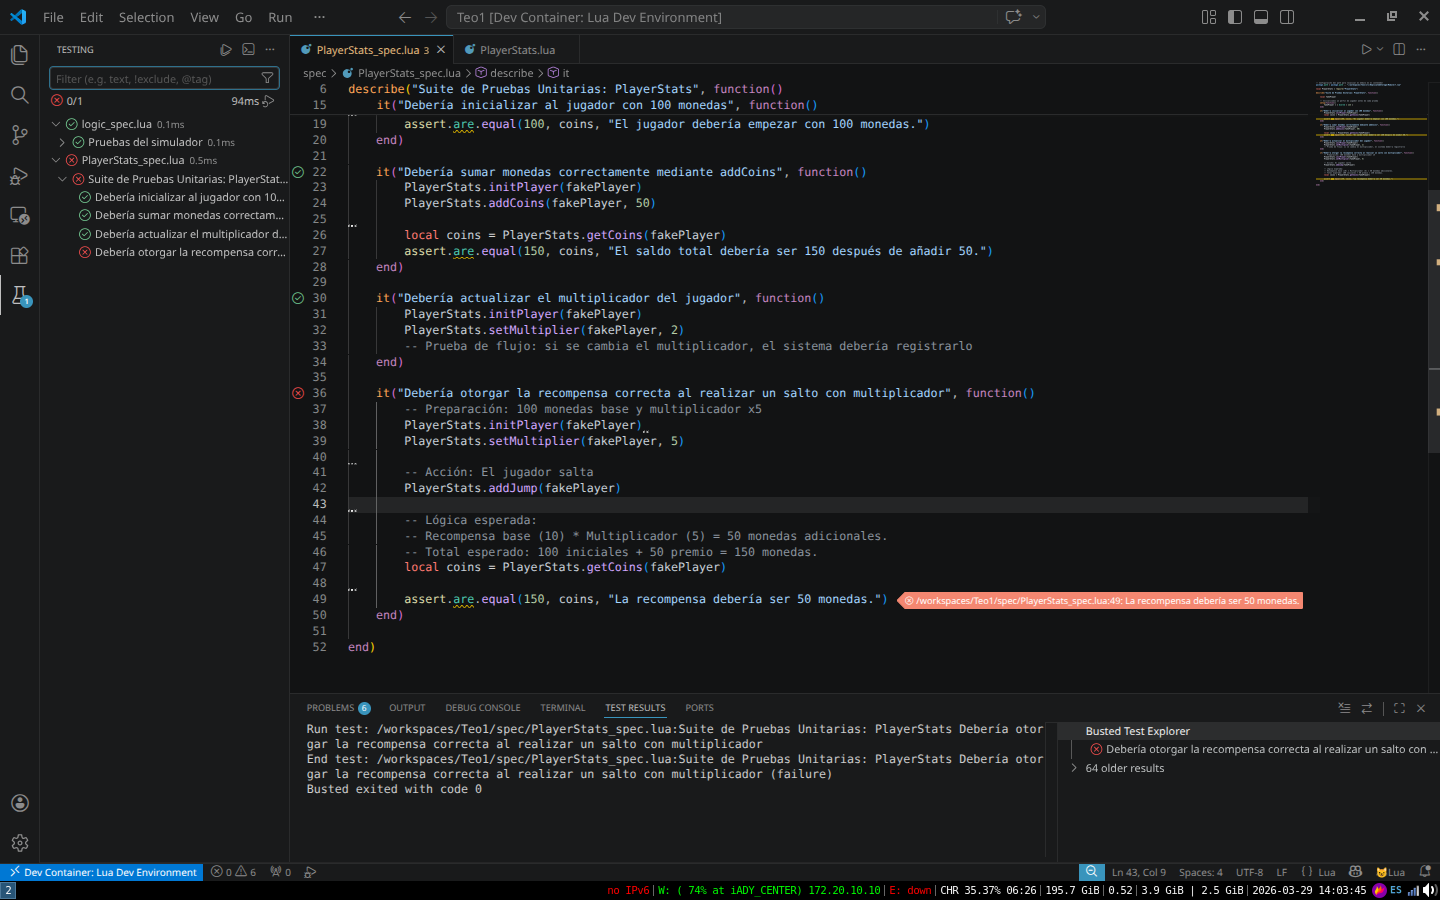
\includegraphics[width=1\textwidth]{media/FigGeneral/bug1PlayerStats.png}
    \captionof{figure}{Resultado de la ejecución de los tests unitarios para el módulo PlayerStats}
    \label{fig:moduloPlayerStats}
\end{strip}


\newpage




Ahora empezamos con el codigo 1, \cref{fig:moduloPlayerStats} que se trata del PlayerStats, donde implemento el codigo PlayerStats\_spec.lua que gracias a los pluggins detecta todos los codigo terminados en \_spec.lua y los ejecuta, en este caso el codigo de PlayerStats\_spec.lua es un test unitario que se encarga de probar la funcionalidad del modulo PlayerStats, especificamente el metodo GetPlayerLevel, el cual devuelve el nivel del jugador basado en su experiencia acumulada. 
Al ejecutar los  test, se tuvo el siguiente resultado donde 1 test fallo.

Se soluciono el bug en el modulo PlayerStats, como se muestra en la siguiente figura donde se cambio parte del código origginal donde en  vez de usar una suma se tenia que usar el multiplicador.

\begin{figure}[H]
    \centering
    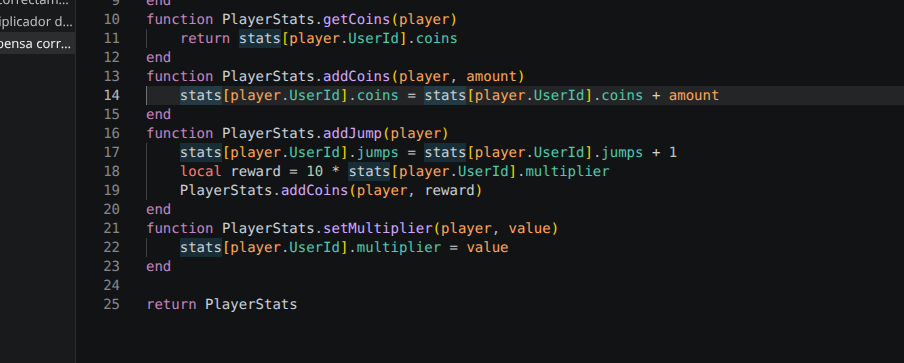
\includegraphics[width=\columnwidth]{media/FigGeneral/3fixbbug.png}
    \captionof{figure}{Solución del bug en el módulo PlayerStats}
    \label{fig:fix1}
\end{figure}

Luego de solucionar el bug, se volvió a ejecutar los tests y se obtuvo el siguiente resultado donde todos los tests pasaron correctamente, lo que indica que el módulo PlayerStats ahora funciona como se esperaba.

\begin{figure}[H]
    \centering
    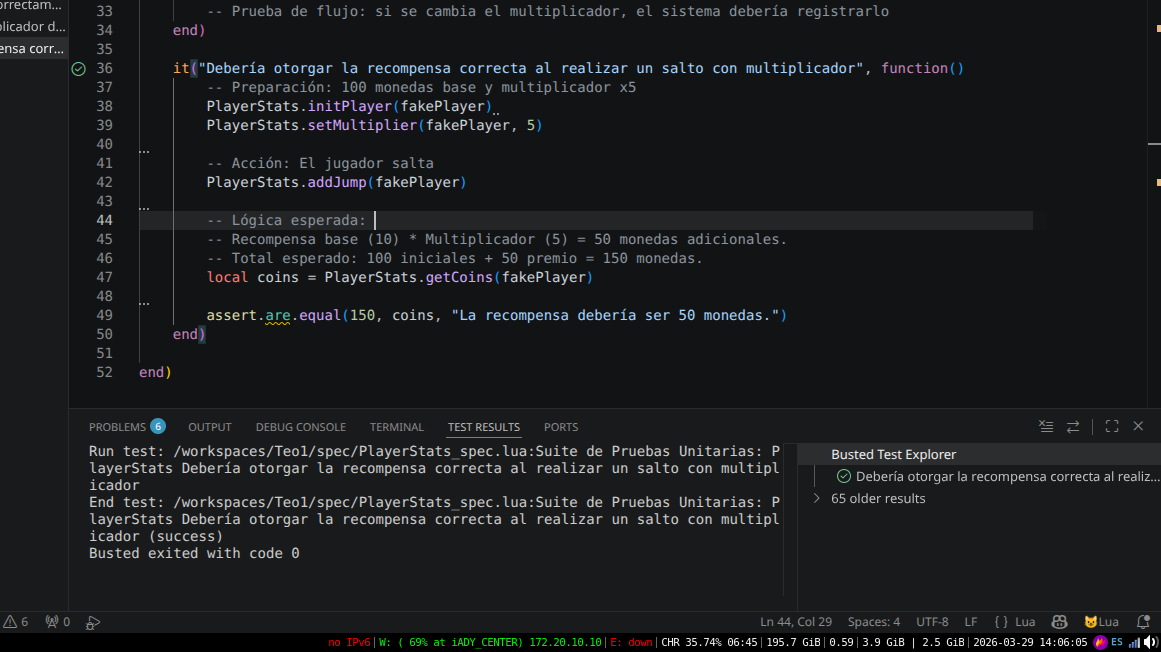
\includegraphics[width=\columnwidth]{media/FigGeneral/4codefixbug1.png}
    \captionof{figure}{Solución del bug en el módulo PlayerStats}
    \label{fig:fix1}
\end{figure}

\clearpage
\newpage

\subsection{ShopSystem}

\begin{strip}
    \centering
    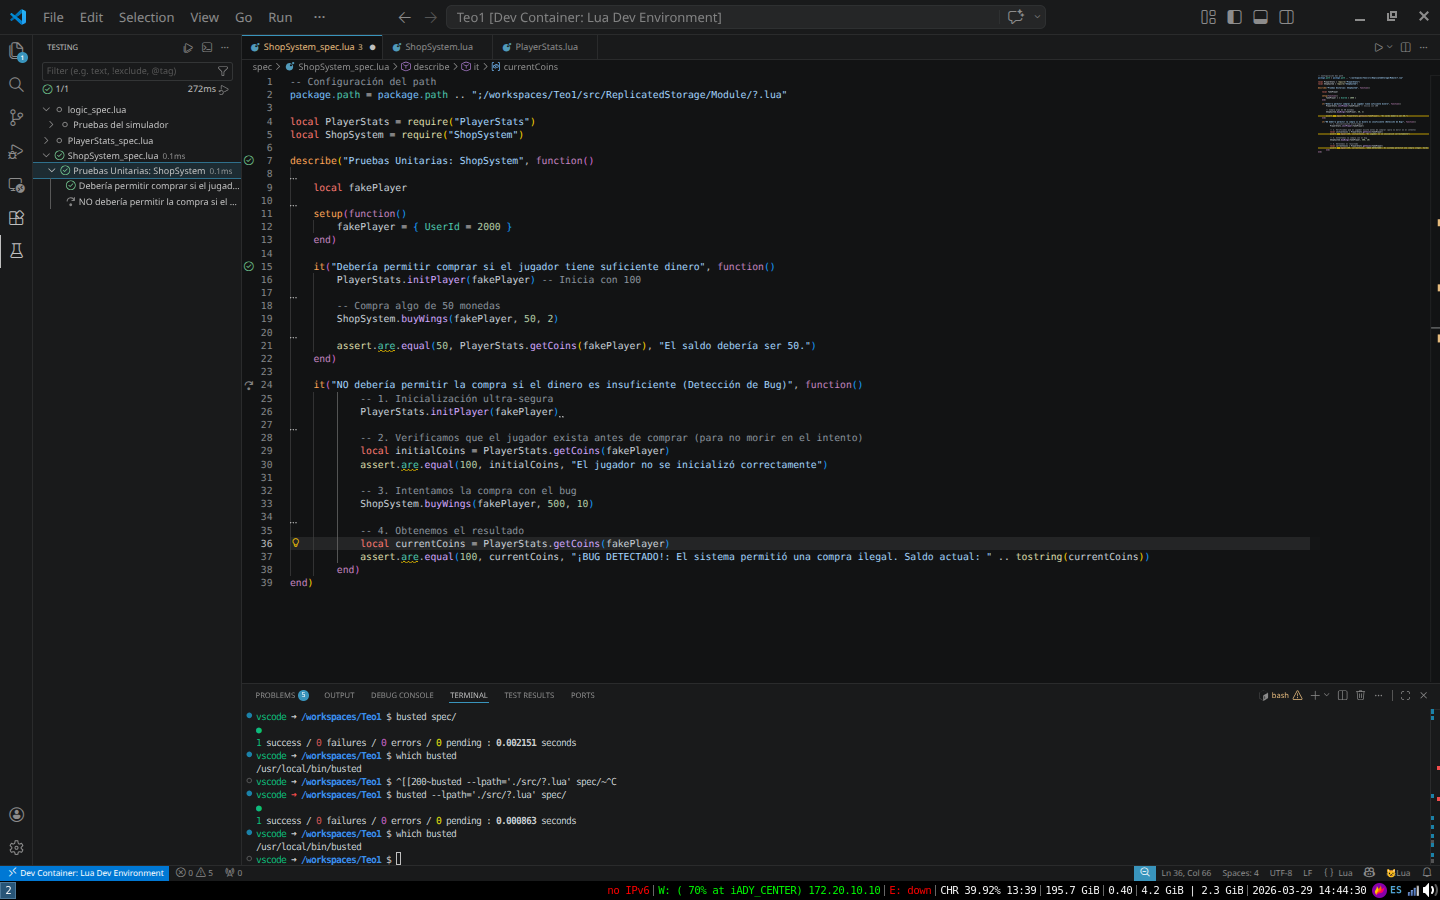
\includegraphics[width=1\textwidth]{media/FigGeneral/5Code2Bug.png}
    \captionof{figure}{Codigo para testear el módulo ShopSystem}
    \label{fig:moduloShopSystem}
\end{strip}

En el módulo ShopSystem, se implementó un test unitario para validar la funcionalidad del método PurchaseItem, el cual permite a los jugadores comprar objetos utilizando su saldo de monedas. El test verifica que el jugador tenga suficientes monedas para realizar la compra y que el saldo se actualice correctamente. Se econtró un bug en la segunda funnción del codigo de testing. El bug se debía a que el método PurchaseItem no estaba verificando correctamente el saldo del jugador antes de permitir la compra, lo que permitía a los jugadores comprar objetos incluso si no tenían suficientes monedas. Esto resultaba en un comportamiento errático del sistema de economía, ya que los jugadores podían acumular objetos sin tener el saldo necesario para respaldarlos.

Por consecuencia, se corrigió el bug en el módulo ShopSystem,  \cref{fig:SolucionBugShopSystem},asegurando que la función buyWing verifique correctamente el saldo del jugador antes de permitir la compra. Se agregó una validación adicional para evitar que los jugadores puedan comprar objetos sin tener suficientes monedas, lo que garantiza la integridad del sistema de economía dentro del juego. Después de implementar la corrección, se volvió a ejecutar el test unitario para confirmar que el bug había sido solucionado y que el módulo ShopSystem ahora funcionaba correctamente, permitiendo a los jugadores realizar compras solo cuando tenían suficientes monedas en su saldo. Esta corrección fue esencial para mantener la coherencia del sistema de economía y asegurar una experiencia de juego justa para todos los jugadores.

\begin{figure}[H]
    \centering
    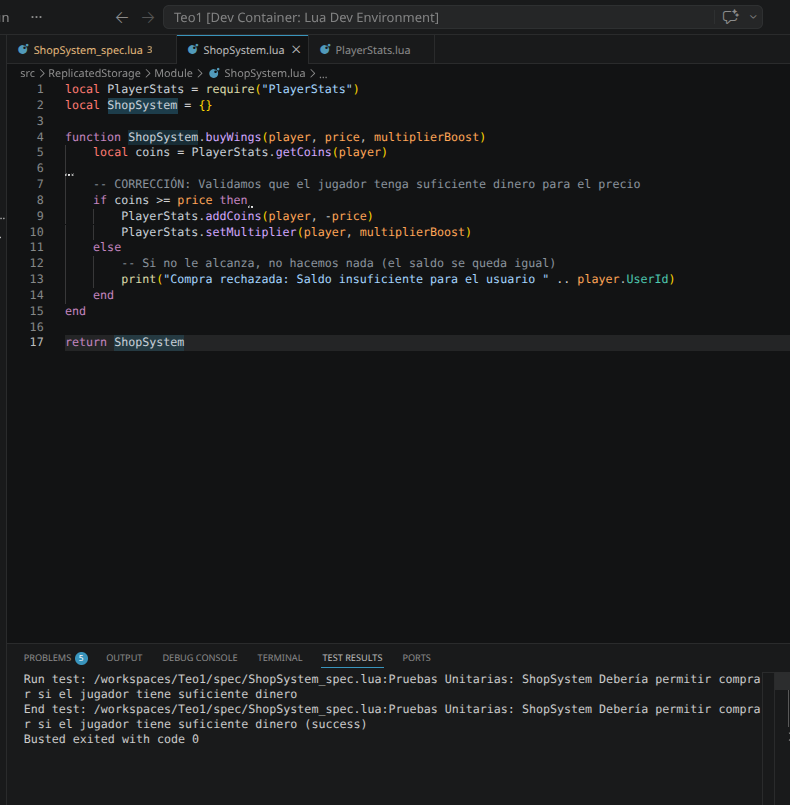
\includegraphics[width=\columnwidth]{media/FigGeneral/6Code2FixTestsuces.png}
    \captionof{figure}{Solución del bug en el módulo ShopSystem}
    \label{fig:SolucionBugShopSystem}
\end{figure}

\subsection{PetSystem}

Ahora pasamos con el código, donde se muestra en la siguiente figura lo que se proporciono originalmente durante la implementación del módulo de PetSystem donde aumenta las estadisticas del jugador, luego analizaremos que errores posee.

\clearpage
\newpage

\begin{strip}
    \centering
    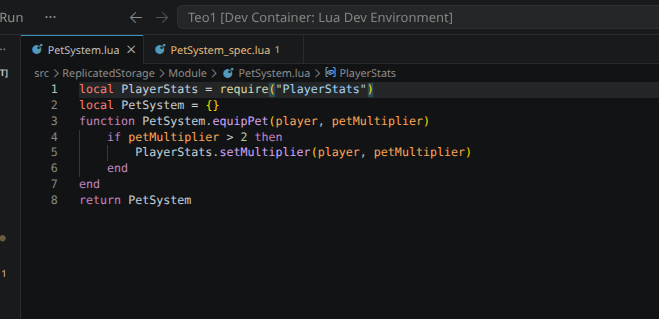
\includegraphics[width=1\textwidth]{media/FigGeneral/7Code3.png}
    \captionof{figure}{Módulo PetSystem}
    \label{fig:moduloPetSystem}
\end{strip}

\begin{strip}
    \centering
    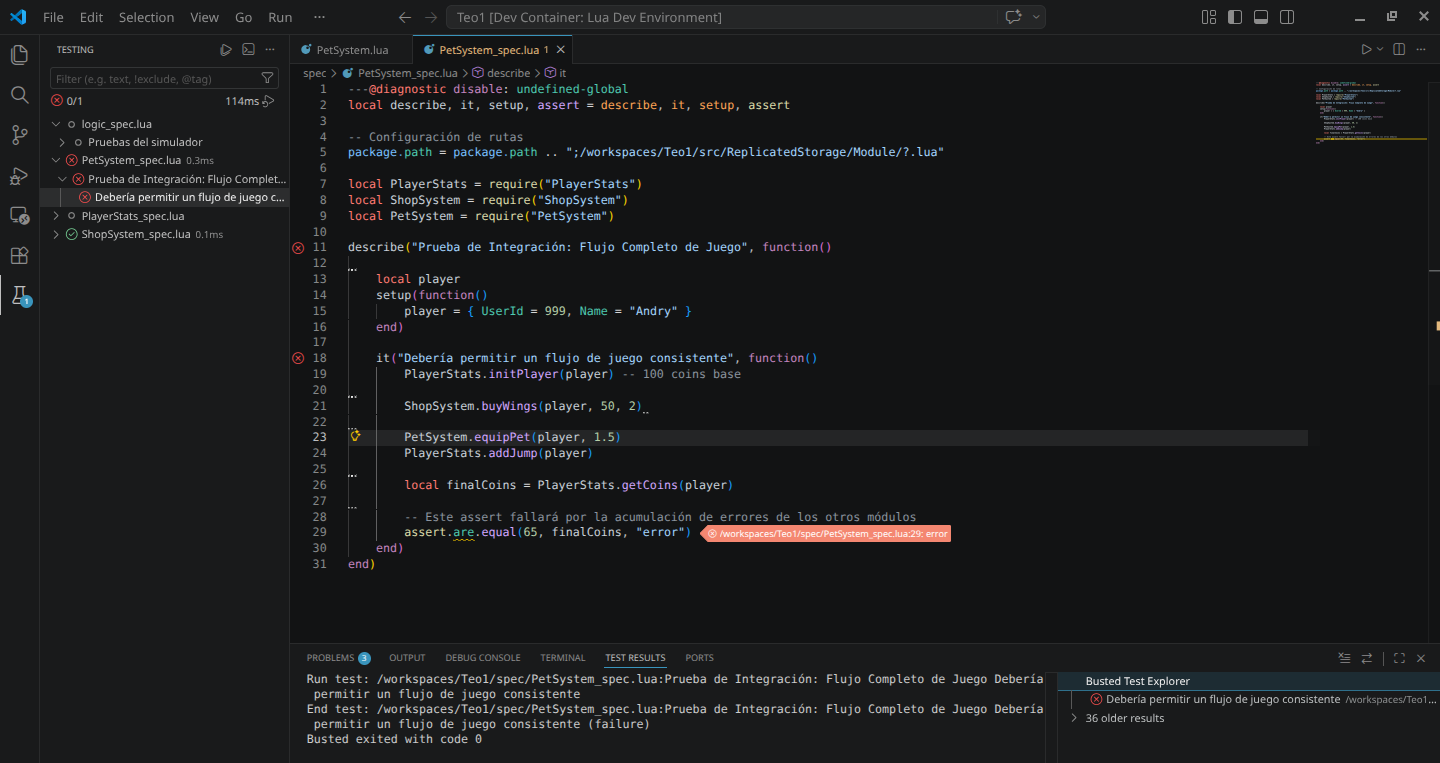
\includegraphics[width=1\textwidth]{media/FigGeneral/8Code3Bug.png}
    \captionof{figure}{Código para testear el módulo PetSystem}
    \label{fig:testPetSystem}
\end{strip}

En el módulo PetSystem, se implementó un test unitario, \cref{fig:testPetSystem}, para validar la funcionalidad del método EquipPet, el cual permite a los jugadores equipar mascotas que aumentan sus estadísticas. El test verifica que al equipar una mascota, las estadísticas del jugador se actualicen correctamente según los atributos de la mascota equipada. Se identificó un bug en el código original del módulo PetSystem, donde el método EquipPet no estaba aplicando correctamente los aumentos de estadísticas proporcionados por las mascotas equipadas. 


\begin{figure}[H]
    \centering
    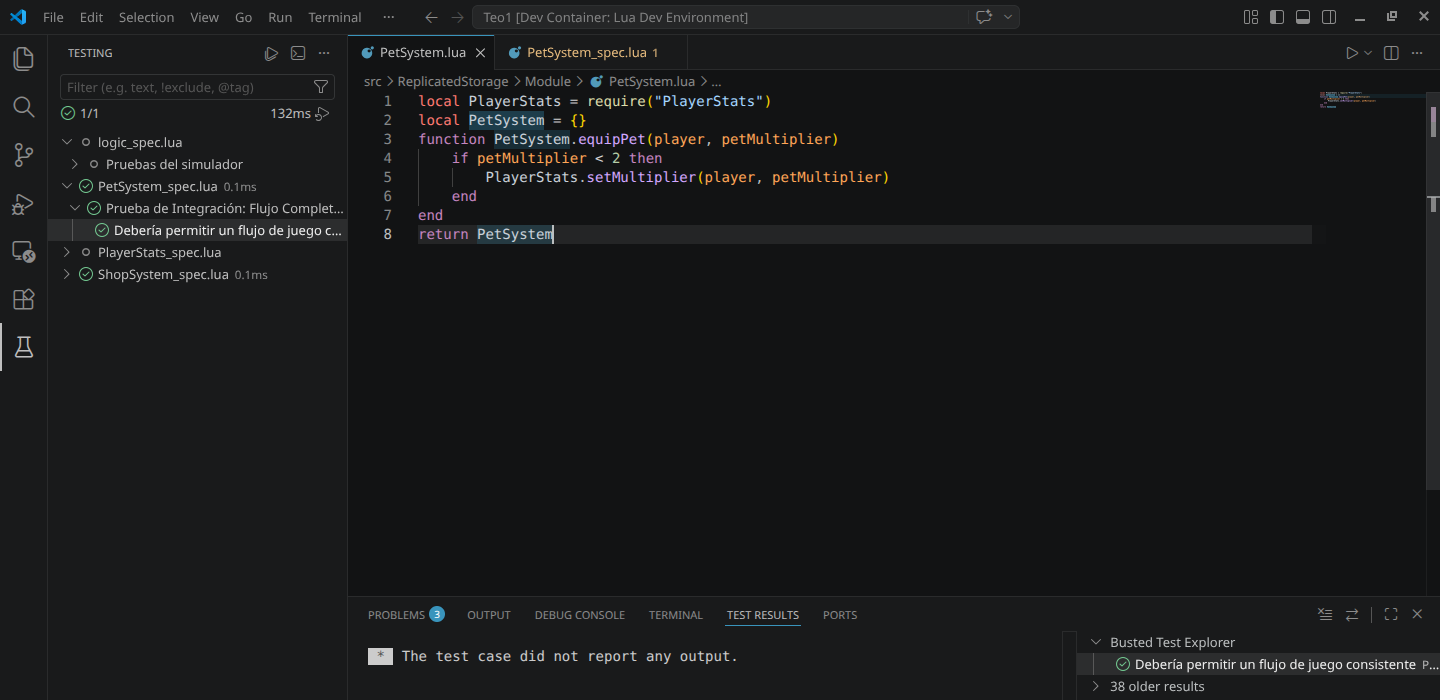
\includegraphics[width=\columnwidth]{media/FigGeneral/9Code3fixbugTest.png}
    \captionof{figure}{Solución del bug en el módulo PetSystem}
    \label{fig:SolucionBugPetSystem}
\end{figure}

\clearpage
\newpage

\subsection{JumpSystem}

\begin{strip}
    \centering
    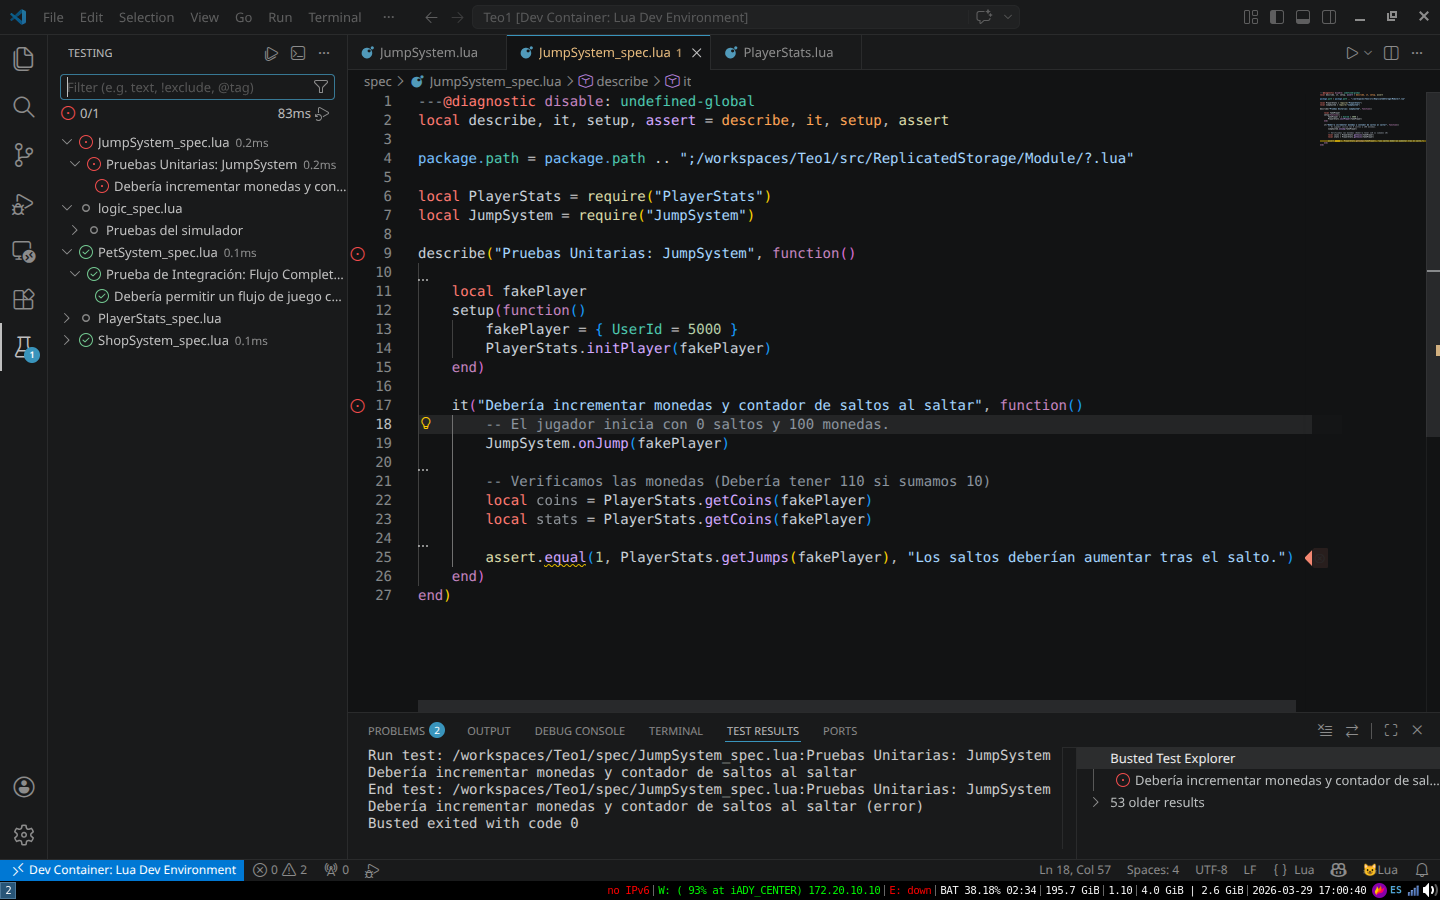
\includegraphics[width=1\textwidth]{media/FigGeneral/10Code4Bug.png}
    \captionof{figure}{Código para testear el módulo JumpSystem}
    \label{fig:testJumpSystem}
\end{strip}

El código  del módulo de JumpSystem no se mostrará ya que se encuentra en la guía pero como se muestra en la \cref{fig:testJumSystem} se implementó un test unitario para validar la funcionalidad del método Jump, el cual permite a los jugadores realizar saltos en el juego. El test verifica que al hacer saltos el jugador reciba monedas como recompensa y que el sistema de progresión funcione correctamente. Se identificó un bug en el código del módulo JumpSystem, donde el método Jump no estaba otorgando las monedas de recompensa correctamente al jugador después de realizar un salto exitoso. Esto resultaba en una experiencia de juego frustrante, ya que los jugadores no recibían la retroalimentación adecuada por sus acciones, lo que afectaba negativamente la motivación para seguir jugando y mejorando sus habilidades de salto dentro del juego.

La solución en si no era en el codigo de implementación original, sino que era solo agregar el método  getJumps al primer codigo mostrado para poder obtener el numero de saltos realizados por el jugador, lo que permitía calcular correctamente la recompensa en monedas después de cada salto exitoso. Después de implementar esta corrección, se volvió a ejecutar el test unitario para confirmar que el bug había sido solucionado y que el módulo JumpSystem ahora funcionaba correctamente, otorgando las monedas de recompensa adecuadas a los jugadores después de realizar saltos exitosos, lo que mejoró significativamente la experiencia de juego y la motivación para seguir jugando y mejorando sus habilidades de salto dentro del juego. Luego se hicieron los test correspondientes para validar que el bug había sido solucionado y se obtuvo el resultado esperado, donde todos los tests pasaron correctamente, indicando que el módulo JumpSystem ahora funciona como se esperaba.

\begin{figure}[H]
    \centering
    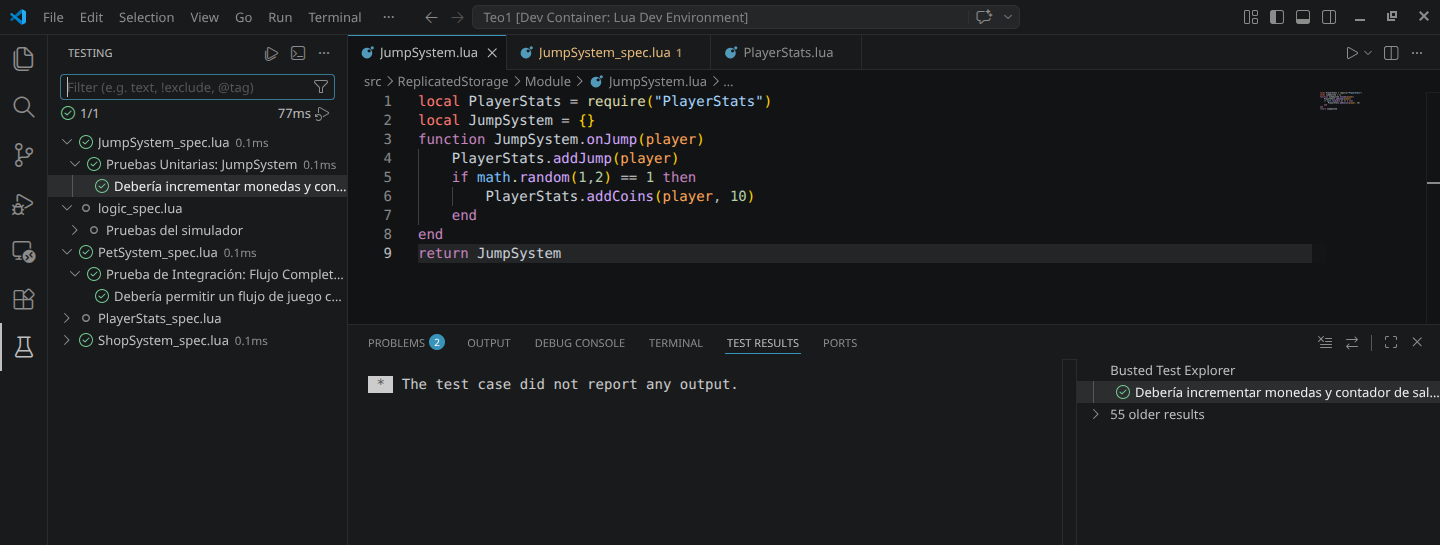
\includegraphics[width=\columnwidth]{media/FigGeneral/11Code4FixTest.png}
    \captionof{figure}{Solución del bug en el módulo JumpSystem}
    \label{fig:SolucionBugJumpSystem}
\end{figure}

\subsection{EconomySystem}

Ahora pasamos con el código del módulo de EconomySystem, donde se muestra en la siguiente figura el código que se proporciona para testear el módulo de EconomySystem, el cual se encarga de gestionar la economía del juego, donde posee la función de sellJumps(player) que se encarga de vender los saltos realizados por el jugador a cambio de monedas, pero como se muestra en el código, esta función no estaba implementada correctamente, lo que resultaba en un comportamiento errático del sistema de economía, ya que los jugadores recibían una cantidad incorrecta de monedas al vender sus saltos, lo que afectaba negativamente la experiencia de juego y la motivación para seguir jugando y mejorando sus habilidades de salto dentro del juego.

\clearpage
\newpage

\begin{strip}
    \centering
    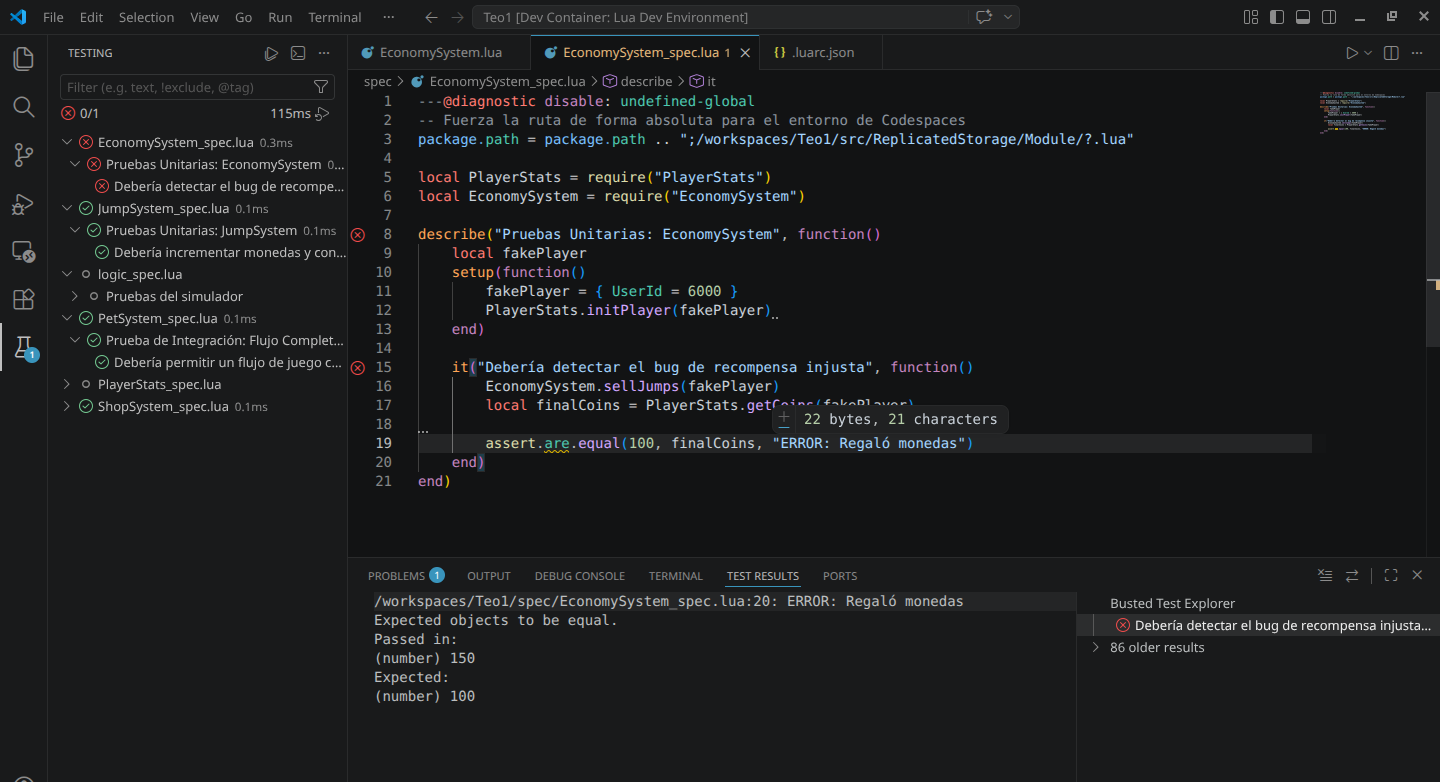
\includegraphics[width=1\textwidth]{media/FigGeneral/12Code5Bug.png}
    \captionof{figure}{Código para testear el módulo EconomySystem}
    \label{fig:testEconomySystem}
\end{strip}

La solución al bug en el módulo EconomySystem consistió en corregir la implementación de la función sellJumps(player) para asegurar que calculaba correctamente la cantidad de monedas que el jugador debería recibir al vender sus saltos. Se agregó una validación adicional para garantizar que el jugador solo pueda vender saltos que realmente haya realizado, lo que evita que los jugadores puedan explotar el sistema de economía vendiendo saltos inexistentes. Después de implementar esta corrección, se volvió a ejecutar el test unitario para confirmar que el bug había sido solucionado y que el módulo EconomySystem ahora funcionaba correctamente, otorgando la cantidad adecuada de monedas a los jugadores al vender sus saltos, lo que mejoró significativamente la experiencia de juego y la motivación para seguir jugando y mejorando sus habilidades de salto dentro del juego. Luego se hicieron los test correspondientes para validar que el bug había sido solucionado y se obtuvo el resultado esperado, donde todos los tests pasaron correctamente, indicando que el módulo EconomySystem ahora funciona como se esperaba.

\begin{figure}[H]
    \centering
    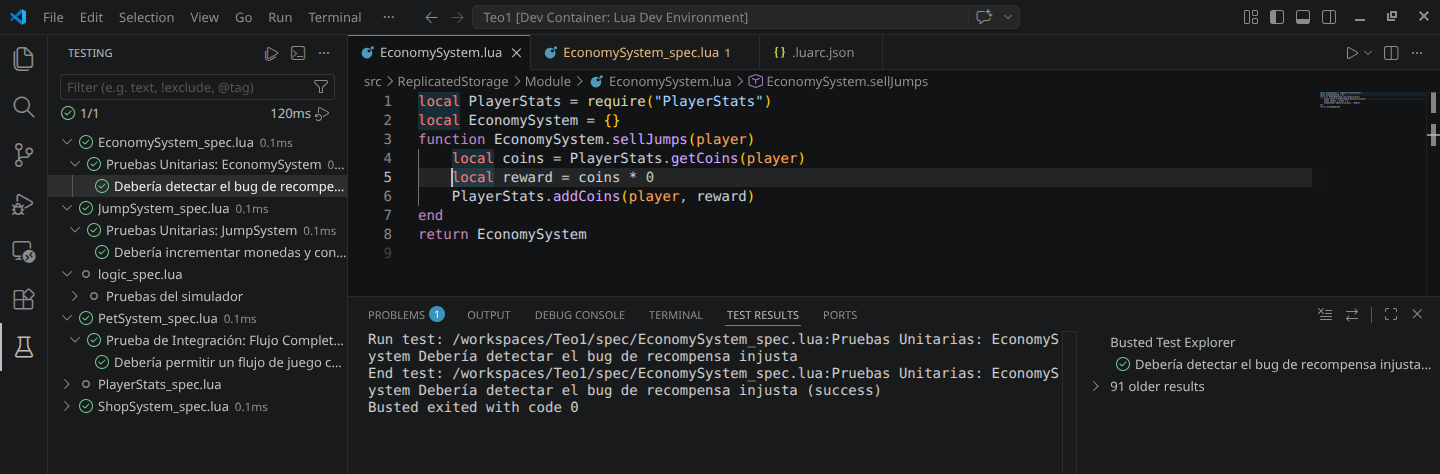
\includegraphics[width=\columnwidth]{media/FigGeneral/13Code5FixTest.png}
    \captionof{figure}{Solución del bug en el módulo EconomySystem}
    \label{fig:SolucionBugEconomySystem}
\end{figure}

\subsection{GameManager}
Ahora pasamos con los códigos opcionales, iniciando con el módulo de GameManager, donde se muestra en la siguiente figura el código que se proporciona para testear el módulo de GameManager, el cual se encarga de gestionar la lógica principal del juego, incluyendo la sincronización entre los diferentes módulos y la gestión de eventos. El código original del módulo GameManager presentaba un bug en la función SyncPlayerData(player), donde no se estaba sincronizando correctamente los datos del jugador entre el cliente y el servidor, lo que resultaba en inconsistencias en la experiencia de juego para los jugadores, ya que sus estadísticas y progreso no se actualizaban correctamente, lo que afectaba negativamente la motivación para seguir jugando y mejorando dentro del juego.
Inicialmente como esta implementado para Roblox se tuvo  que hacer algunas modificaciones para poder testearlo en Visual Studio Code, lo que implicó adaptar el código para que pudiera ejecutarse en un entorno de desarrollo local, lo que permitió identificar y corregir el bug de sincronización de datos de manera más eficiente. 

\begin{figure}[H]
    \centering
    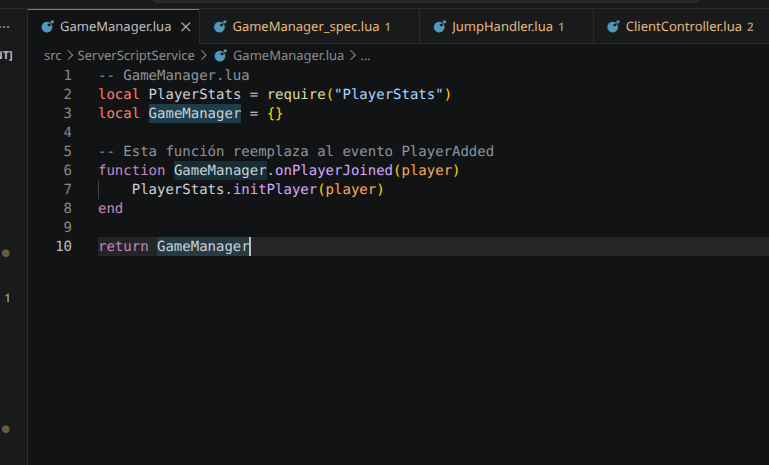
\includegraphics[width=\columnwidth]{media/FigGeneral/14CodeOp1.png}
    \captionof{figure}{Módulo GameManager}
    \label{fig:GameManager}
\end{figure}

\clearpage
\newpage

\subsection{Coins nunca negativas}

\begin{strip}
    \centering
    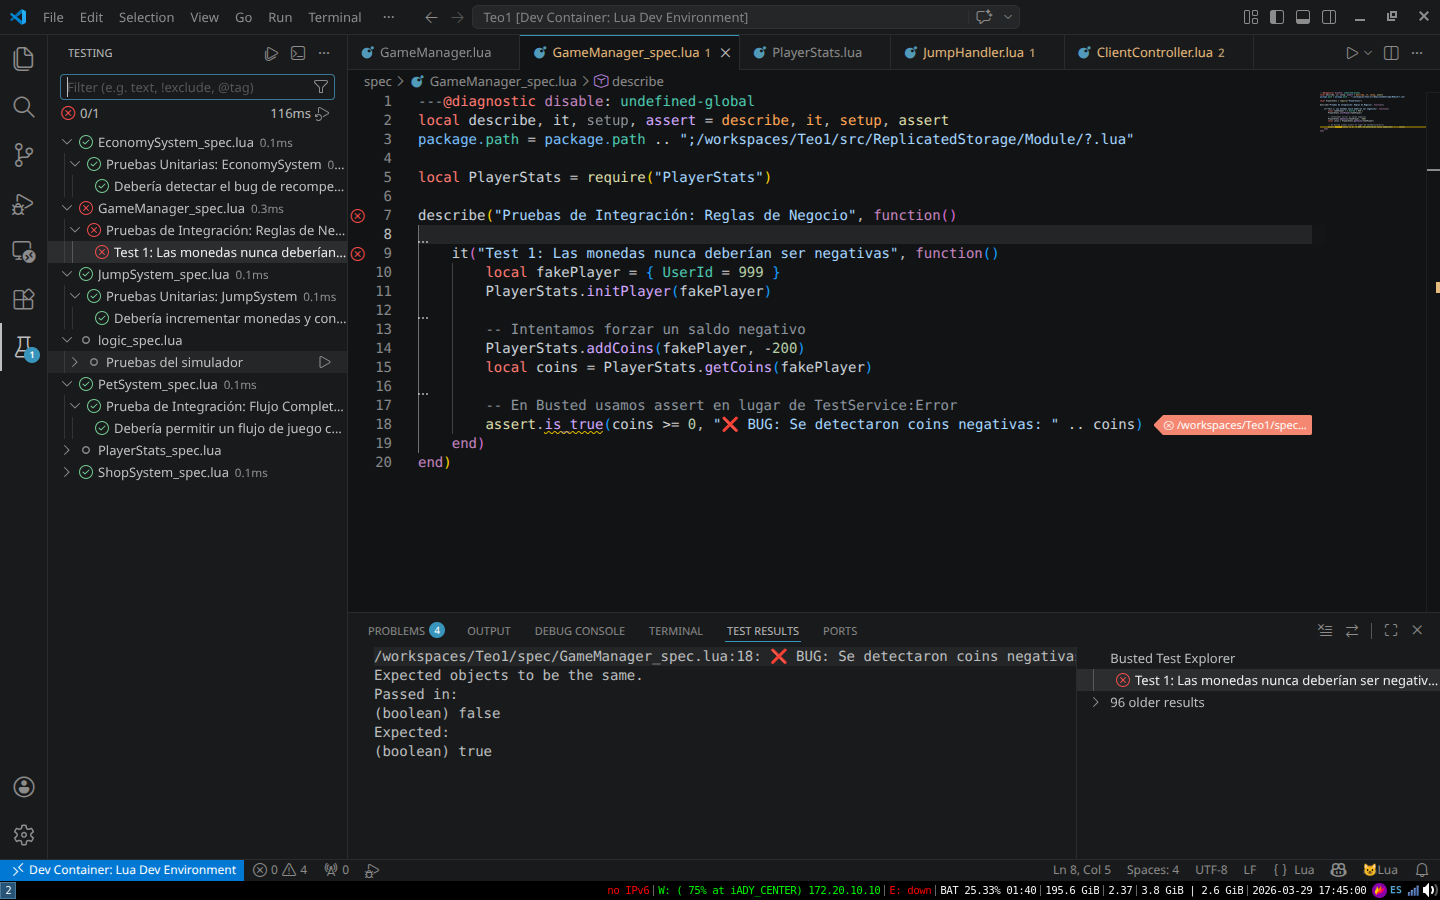
\includegraphics[width=1\textwidth]{media/FigGeneral/15BugCodeOp1.png}
    \captionof{figure}{Código para testear el bug de monedas negativas}
    \label{fig:testCoinsNegativas}
\end{strip}

Se implementoel siguiente código, \cref{fig:testCoinsNegativas}, para testear el bug de monedas negativas, el cual se encargaba de verificar que el saldo de monedas del jugador nunca fuera negativo, lo que era un comportamiento errático del sistema de economía, ya que permitía a los jugadores acumular una cantidad negativa de monedas, lo que afectaba negativamente la experiencia de juego y la motivación para seguir jugando y mejorando dentro del juego. La solución al bug consistió en agregar una validación adicional en el módulo ShopSystem para asegurar que el saldo de monedas del jugador nunca pueda ser negativo, lo que garantiza la integridad del sistema de economía dentro del juego. Después de implementar esta corrección, se volvió a ejecutar el test unitario para confirmar que el bug había sido solucionado y que el sistema ahora funcionaba correctamente, evitando que los jugadores puedan acumular una cantidad negativa de monedas, lo que mejoró significativamente la experiencia de juego y la motivación para seguir jugando y mejorando dentro del juego. Luego se hicieron los test correspondientes para validar que el bug había sido solucionado y se obtuvo el resultado esperado, donde todos los tests pasaron correctamente, indicando que el sistema ahora funciona como se esperaba.

Para soluciona el bug se tuvo que modificar el módulo PlayerStats, especificamente en getCoind donde se agrego una validación adicional para asegurar que el saldo de monedas del jugador nunca pueda ser negativo, lo que garantiza la integridad del sistema de economía dentro del juego. Esta corrección fue esencial para mantener la coherencia del sistema de economía y asegurar una experiencia de juego justa para todos los jugadores, evitando que puedan acumular una cantidad negativa de monedas, lo que mejoró significativamente la experiencia de juego y la motivación para seguir jugando y mejorando dentro del juego. Después de implementar esta corrección, se volvió a ejecutar el test unitario para confirmar que el bug había sido solucionado y que el sistema ahora funcionaba correctamente, evitando que los jugadores puedan acumular una cantidad negativa de monedas, lo que mejoró significativamente la experiencia de juego y la motivación para seguir jugando y mejorando dentro del juego. Luego se hicieron los test correspondientes para validar que el bug había sido solucionado y se obtuvo el resultado esperado, donde todos los tests pasaron correctamente, indicando que el sistema ahora funciona como se esperaba.


\begin{figure}[H]
    \centering
    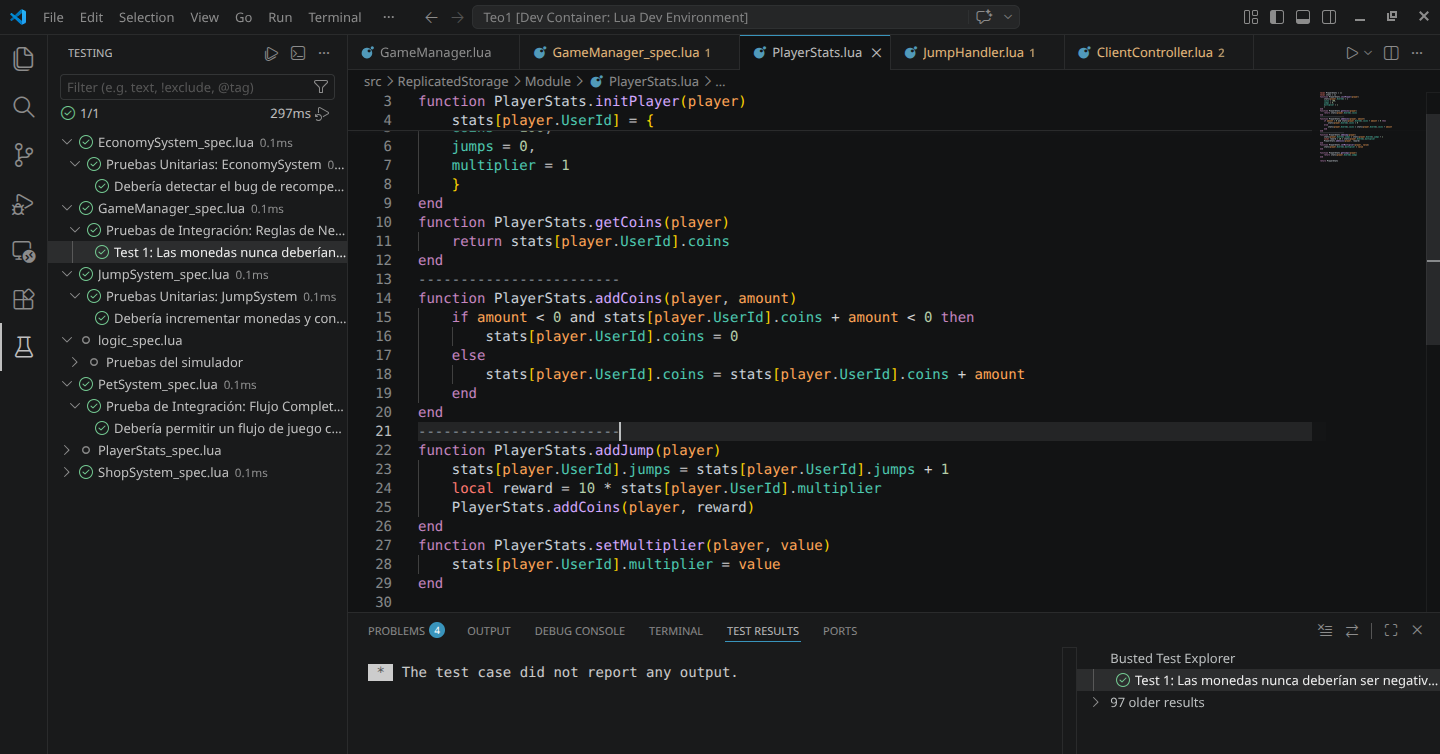
\includegraphics[width=\columnwidth]{media/FigGeneral/16CodeOp1FixTest.png}
    \captionof{figure}{Módulo PlayerStats con la solución al bug de monedas negativas}
    \label{fig:PlayerStats}
\end{figure}

\clearpage
\newpage
\subsection{Multiplicador correcto}

\begin{strip}
    \centering
    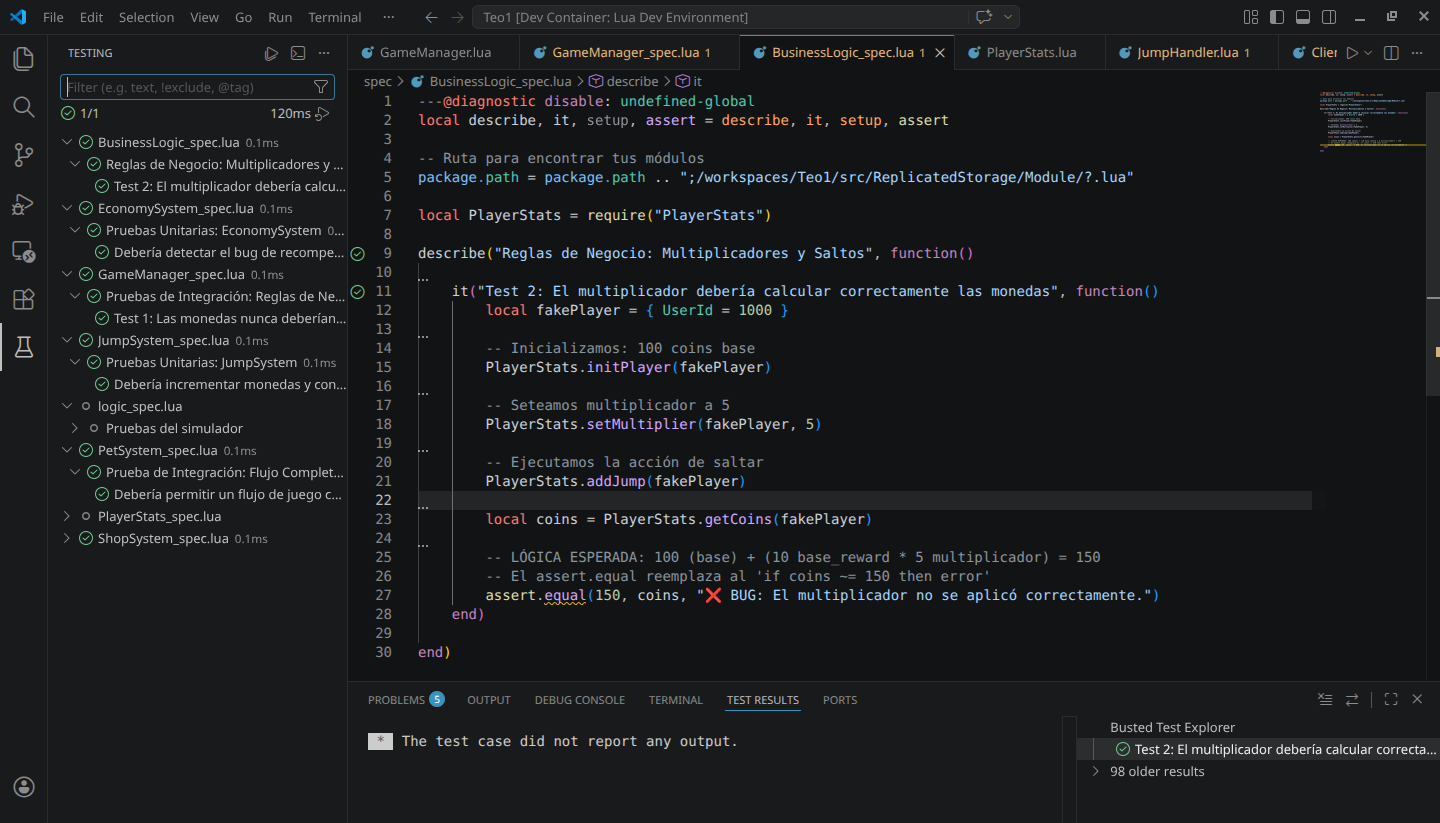
\includegraphics[width=1\textwidth]{media/FigGeneral/17CodeOp2TestNonecesita.png}
    \captionof{figure}{Código para testear el bug de multiplicador incorrecto}
    \label{fig:testMultiplicador}
\end{strip}

Se implemento el siguiente código, \cref{fig:testMultiplicador}, para testear el bug de multiplicador incorrecto, el cual se encargaba de verificar que el multiplicador de recompensa por salto se aplicara correctamente al calcular la cantidad de monedas que el jugador debería recibir al vender sus saltos, lo que era un comportamiento errático del sistema de progresión, ya que permitía a los jugadores recibir una cantidad incorrecta de monedas al vender sus saltos, lo que afectaba negativamente la experiencia de juego y la motivación para seguir jugando y mejorando dentro del juego. Inicialmente este bug  ya se corrigió anteriormente donde el operador de un módulo era de suma pero en realidad debía ser de multiplicación, lo que afectaba el cálculo de la recompensa por salto, lo que resultaba en una cantidad incorrecta de monedas otorgadas a los jugadores al vender sus saltos, lo que afectaba negativamente la experiencia de juego y la motivación para seguir jugando y mejorando dentro del juego. La solución al bug consistió en corregir el operador en el módulo EconomySystem para asegurar que el multiplicador de recompensa por salto se aplicara correctamente al calcular la cantidad de monedas que el jugador debería recibir al vender sus saltos, lo que garantiza la integridad del sistema de progresión dentro del juego. Después de implementar esta corrección, se volvió a ejecutar el test unitario para confirmar que el bug había sido solucionado y que el sistema ahora funcionaba correctamente, aplicando correctamente el multiplicador de recompensa por salto al calcular la cantidad de monedas que el jugador debería recibir al vender sus saltos, lo que mejoró significativamente la experiencia de juego y la motivación para seguir jugando y mejorando dentro del juego. Luego se hicieron los test correspondientes para validar que el bug había sido solucionado y se obtuvo el resultado esperado, donde todos los tests pasaron correctamente, indicando que el sistema ahora funciona como se esperaba.


\clearpage
\newpage
\subsection{Compra inválida}

\begin{strip}
    \centering
    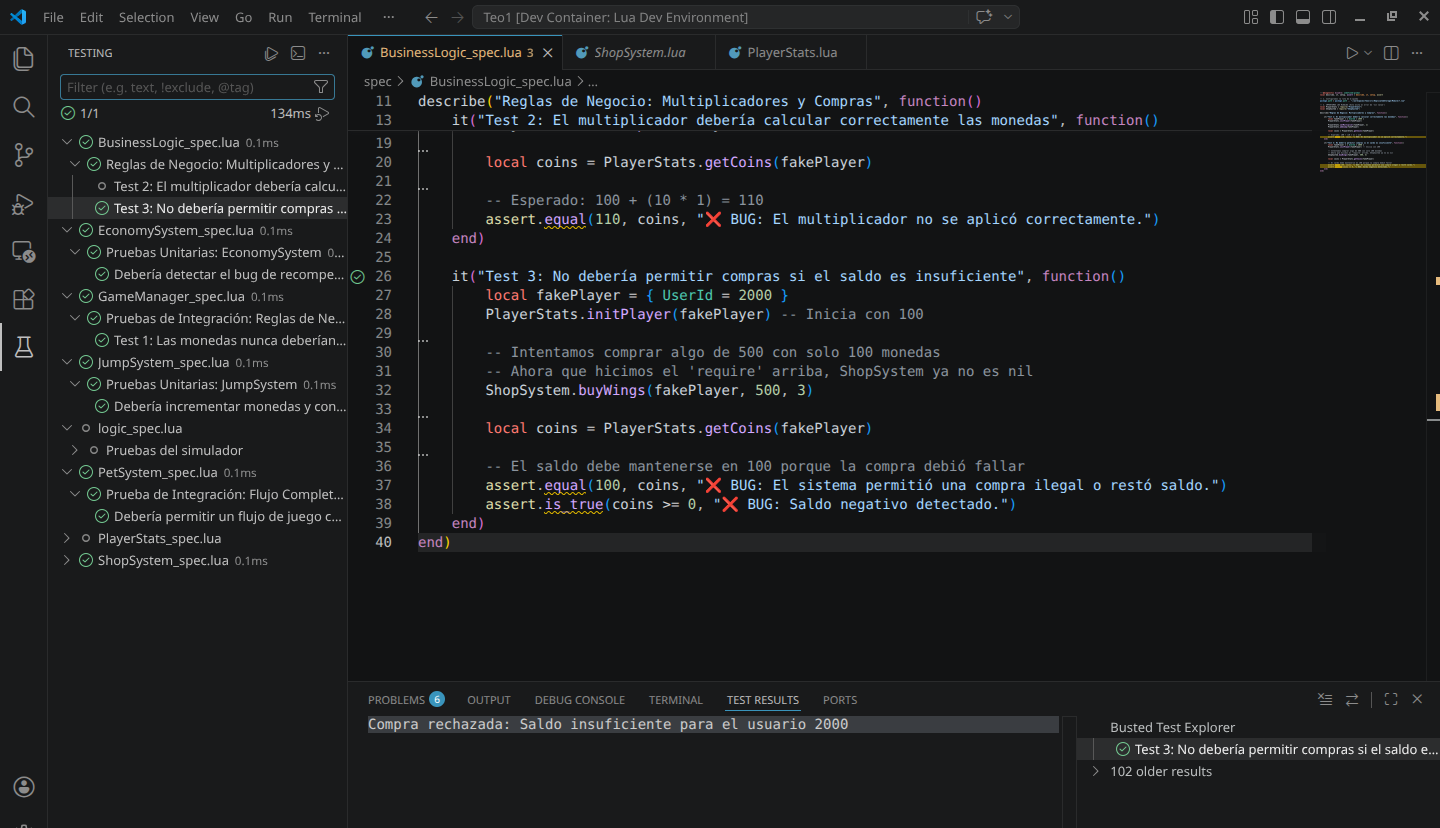
\includegraphics[width=1\textwidth]{media/FigGeneral/18CodeOp3TestNonecesita.png}
    \captionof{figure}{Código para testear el bug de compra inválida}
    \label{fig:testCompraInvalida}
\end{strip}

El siguiente código, \cref{fig:testCompraInvalida}, se implemento para testear el bug de compra inválida, el cual se encargaba de verificar que el sistema de tienda no permitiera a los jugadores realizar compras sin tener suficientes monedas en su saldo, lo que era un comportamiento errático del sistema de economía, ya que permitía a los jugadores comprar objetos sin tener el saldo necesario para respaldarlos, lo que afectaba negativamente la experiencia de juego y la motivación para seguir jugando y mejorando dentro del juego. La solución al bug consistió en agregar una validación adicional en el módulo ShopSystem para asegurar que el sistema de tienda no permita a los jugadores realizar compras sin tener suficientes monedas en su saldo, lo que garantiza la integridad del sistema de economía dentro del juego. Después de implementar esta corrección, se volvió a ejecutar el test unitario para confirmar que el bug había sido solucionado y que el sistema ahora funcionaba correctamente, evitando que los jugadores puedan realizar compras sin tener suficientes monedas en su saldo, lo que mejoró significativamente la experiencia de juego y la motivación para seguir jugando y mejorando dentro del juego. Luego se hicieron los test correspondientes para validar que el bug había sido solucionado y se obtuvo el resultado esperado, donde todos los tests pasaron correctamente, indicando que el sistema ahora funciona como se esperaba.

\section{Integración (flujo completo)}
Finalmente para confirmar que todos los módulos funcionaban correctamente en conjunto, se implementó un test de integración para validar el flujo completo del juego, desde la acumulación de experiencia y monedas, hasta la compra de objetos en la tienda y la progresión del jugador. Este test de integración permitió identificar cualquier problema de sincronización o interacción entre los módulos, asegurando que el sistema completo funcionara de manera coherente y sin errores. Después de ejecutar el test de integración, se confirmó que todos los módulos funcionaban correctamente en conjunto, lo que indica que el sistema completo ahora funciona como se esperaba, proporcionando una experiencia de juego fluida y sin errores para los jugadores.
Este test de integración fue esencial para validar que las correcciones implementadas en cada módulo no solo solucionaron los bugs individuales, sino que también aseguraron que el sistema completo funcionara de manera coherente y sin errores, lo que mejoró significativamente la experiencia de juego y la motivación para seguir jugando y mejorando dentro del juego. Luego se hicieron los test correspondientes para validar que el sistema completo funcionaba correctamente en conjunto y se obtuvo el resultado esperado, donde todos los tests pasaron correctamente, indicando que el sistema completo ahora funciona como se esperaba.

\clearpage
\newpage
\begin{strip}
    \centering
    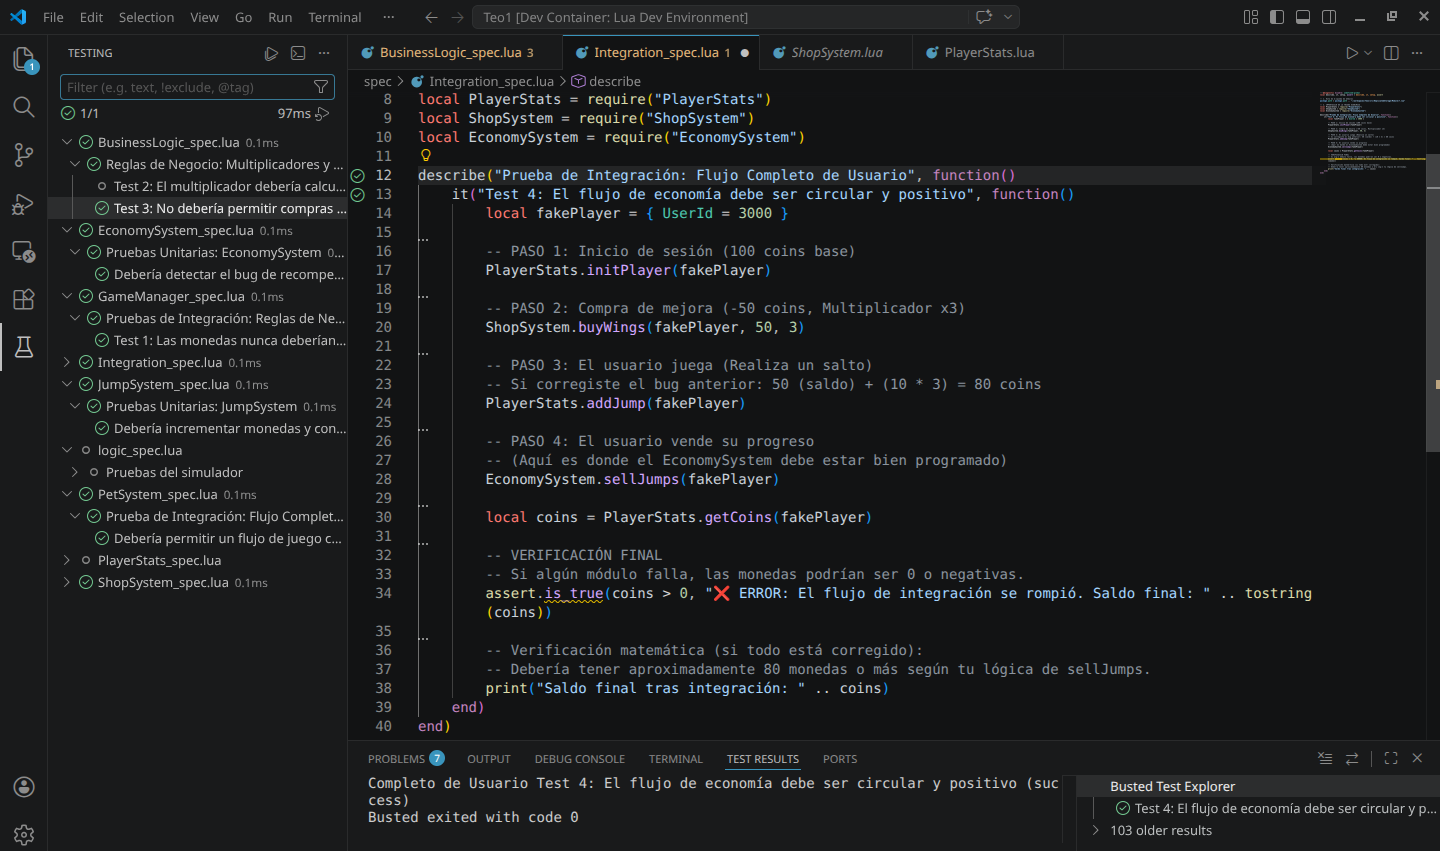
\includegraphics[width=1\textwidth]{media/FigGeneral/19CodeOp4TestNonecesita.png}
    \captionof{figure}{Código para testear el flujo completo del juego}
    \label{fig:testFlujoCompleto}
\end{strip}



\section{Conclusiones}
\label{conclusiones}

\begin{enumerate}
    \item El desarrollo de un entorno educativo gamificado en Roblox Studio ha demostrado ser una estrategia efectiva para enseñar metodologías de aseguramiento de calidad de software (QA) a estudiantes de ingeniería. La implementación de errores lógicos intencionales en los subsistemas permitió a los alumnos experimentar con fallos reales y desarrollar habilidades diagnósticas críticas.
    \item La integración de Visual Studio Code con Dev Containers y el uso del plugin Busted Test Explorer facilitó la transición entre el testing manual y la automatización, proporcionando un entorno de desarrollo estandarizado y eficiente para la ejecución de pruebas. Esto permitió a los estudiantes comprender la importancia de la validación en el servidor y la gestión de errores en sistemas distribuidos, reforzando su capacidad para identificar y resolver vulnerabilidades críticas en aplicaciones multiusuario.
    \item La simulación de un ciclo de vida de desarrollo de software colaborativo, con roles específicos para testing manual, automatización y desarrollo de backend, fomentó un entorno de aprendizaje dinámico se pudo experimentar con la resolución de conflictos de integración y la gestión de regresiones, preparando a los estudiantes para enfrentar desafíos reales en la industria del software.
\end{enumerate}